\section{Introduction}
\label{industry_needs}
As we mentioned in chapter \ref{chapter_general_intro}, the aim of this thesis was twofold: deriving a methodology for inferring the motivational state of individuals while interacting with potentially rewarding object and presenting how this could be used in industry settings for automated engagement prediction.

In this chapter we will focus on sketching the design of a system for employing our methodology in an industry setting. First we will provide an overview of which potential need an industry player (or a collection of) might have with respect to engagement prediction. We will then proceed at illustrating a system designed for serving this needs. Finally we will present how the components of this system connect with the work we presented so far and how can be leveraged for satisfying said needs.

\section{The Needs from the Videogames Industry}
\label{industry_needs}
As we mentioned before despite the industry might be interested in the development of research projects the the focus of this project is less on the advancement of the research field on more focused on the solution of practical problems. 

In this view how does engagement connects with practical problems that the industry has? Very often (if not always) the success of a videogame title is strictly connected with either its ability to retain users or with the experience that users had with the product. The first is pivotal in scenarios where game is treated as a service sold to an audience (similarly to the function of streaming services) while the second is more relevant in scenarios where games are considered digital goods. 

In this context, engagement can be viewed as a measure of how a particular game was, is or will be able to retain users: if an individual is engaged with a particular service it is likely that will keep take advantage of it similarly if an individual had a particular good experience and gladly engaged with a particular digital good it is is more likely that will either suggest it to other users, buy similar products or buy product from the same seller.  

In this view being able to estimate the current propensity of a user towards a specific game translates (in a more or less direct way) to the capacity of assessing if a game is likely to be a success of public and revenue. For this reason it is often the case that videogame publishers and studios try to leverage the information they have available through telemetry system for taking the stock of how a particular game is performing. This is the classical example of analytical reports summarizing various type of game related Key Performance Indicators. 

\section{Some Ethical Consideration}
\label{industry_needs}
Given the widespread use of automated system relying on data generated by individuals, a series of ethical consideration should be made.

First, when realizing a fully automated system relying on machine learned models the issue of fairness should be taken into account. By fairness we entail all the principles raised in the last few years for making sure that the decision based on the outcome of a machine learning model do not inadvertently bring harm to different groups of people. This might realize in the form of biases in the data on which a certain algorithm is fitted or unconstrained predictions are used for decision making.

\section{Multi-context Automated Engagement Prediction and Quantification}
\label{industry_needs}

\section{Data Generation}
\lorem
\section{Model Owner}
\lorem
\subsection{Data Storage}
\lorem
\subsection{Model Generation}
\lorem
\section{Model Consumer}
\lorem
\subsection{Representation Sharing}
\lorem
\subsection{Profile Generation}
\lorem
\subsection{Live Predictions}
\lorem
\subsection{Automated Reporting}
\lorem

\begin{figure}[ht]
\centering
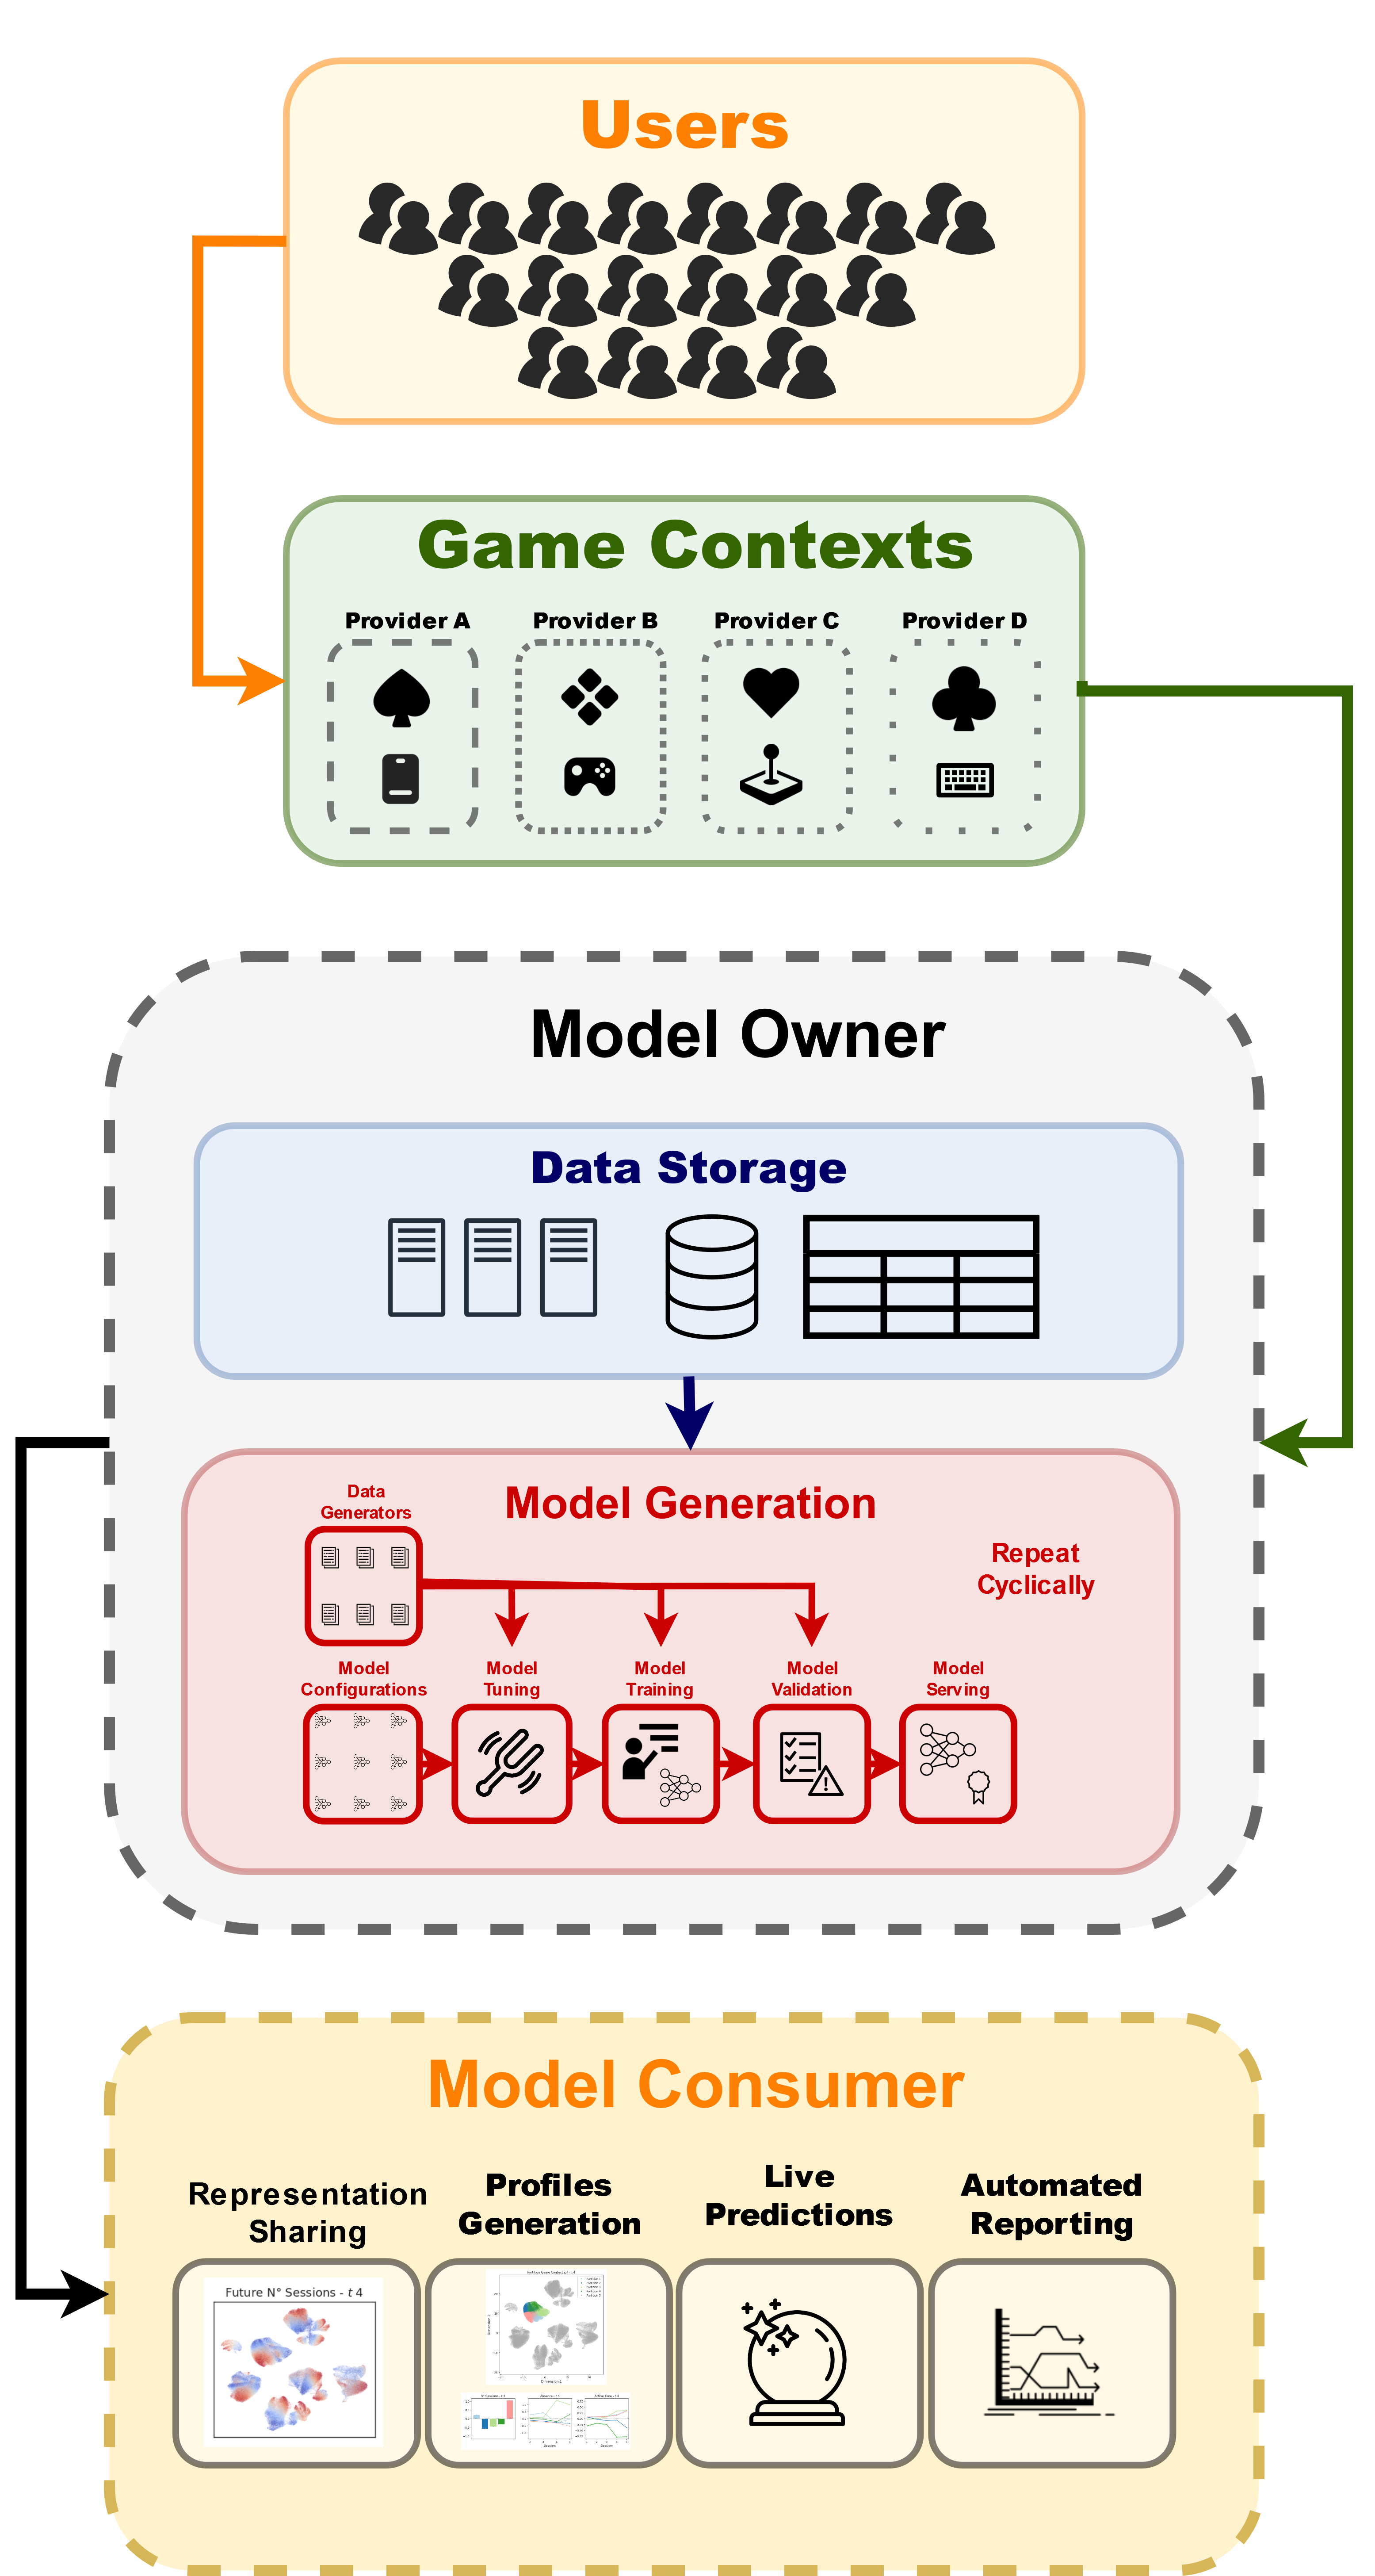
\includegraphics[width=0.7\textwidth]{images/chapter_5/pipeline_diagram.png}
\caption[\textbf{Model Deployment Pipeline}]{The figure represents a simplified system diagram for a potential application of the improved RNN architecture. Solid lines represent low-level components in the system while dashed lines indicate high-level entities. Directional arrows represent the flow of operations inside the system.}
\label{pipeline}
\end{figure}